\section{\twoMode\ $\SOn{2}$-equivariant flow}
\label{s:twoMode}

Dangelmayr,\rf{Dang86} Armbruster, Guckenheimer and Holmes,\rf{AGHO288}
Jones and Proctor,\rf{JoPro87} and Porter and Knobloch\rf{PoKno05} (see
Golubitsky \etal\rf{golubII}, Sect. XX.1) have investigated bifurcations
in 1:2 resonance ODE normal form models to third order in the amplitudes.
Our starting point is such a model
that we shall refer to as the {\twoMode} system:
\bea
	\dot{z}_1 &=& (\mu_1-\ii\, e_1)\,z_1+a_1\,z_1|z_1|^2
				 +b_1\,z_1|z_2|^2+c_1\,\overline{z}_1\,z_2
	\continue
	\dot{z}_2 &=& (\mu_2-\ii\, e_2)\,{z_2}+a_2\,z_2|z_1|^2
				 +b_2\,z_2|z_2|^2+c_2\,z_1^2 \,,
	\label{eq:DangSO2}
\eea
with $z_1,\,z_2$  complex, and all parameters real valued. The complex
\twoMode\ system \refeq{eq:DangSO2} may be rewritten as a 4-dimensional
first order ODE system,
by substitution $z_1 = x_1 + i\,y_1$, $z_2 = x_2 + i\,y_2$,
\bea
\dot{x}_1 &=& (\mu_1 + a_1 r_1^2 + b_1 r_2^2 + c_1 x_2)x_1 + c_1 y_1 y_2 + e_1 y_1
\continue
\dot{y}_1 &=& (\mu_1 + a_1 r_1^2 + b_1 r_2^2 - c_1 x_2)y_1 + c_1 x_1 y_2 - e_1 x_1
\continue
\dot{x}_2 &=& (\mu_2 + a_2 r_1^2 + b_2 r_2^2)x_2 + c_2 (x_1^2 - y_1^2) + e_2 y_2
\continue
\dot{y}_2 &=& (\mu_2 + a_2 r_1^2 + b_2 r_2^2)y_2 + 2 c_2 x_1 y_1 - e_2 x_2
\continue
		  && \mbox{where } r_1^2 = x_1^2 + y_1^2\, , \quad r_2^2 = x_2^2 + y_2^2
\,.
\label{2mode4D}
\eea
As our goal is only to
illustrate and compare continuous symmetry reduction schemes, we shall
study here several simplified versions of model \refeq{2mode4D}, in
the dimensionally lowest possible setting, with the full \statesp\ of
dimension $d=4$, and the $\SOn{2}$-reduced dynamics taking place in 3
dimensions. For these models the
parameters are far from the bifurcation values, and have no
physical interpretation.

It can be checked by inspection that equations \refeq{eq:DangSO2} are
equivariant under the \Un{1}\ transformation
\beq
(z_1,z_2) \rightarrow   (e^{i {\gSpace}}z_1,e^{i 2{\gSpace}} z_2)
\,.
\ee{Dang86(1.1)aa}
In the real representation \refeq{2mode4D}, the $\SOn{2}$ group action
\refeq{Dang86(1.1)aa} is given by $\ssp'= \exp\left( \theta \Lg\right)\ssp$,
where $\transp{\ssp} = \{ x_1, y_1,x_2, y_2\}$, and $\Lg$ is the Lie algebra
generator
\beq
\Lg  \, =
\left( \begin{array}{cccc}
         0 & -1 & 0 & 0 \\
         1 & 0 & 0 & 0 \\
         0 & 0 & 0 & -2\\
         0 & 0 & 2 & 0
      \end{array} \right)
\,.
\ee{LGTwoMode}
One can easily check that the real \twoMode\ system \refeq{2mode4D}
satisfies the equivariance condition \refeq{inftmInv}.

The parameters $\{e_1,e_2\}$ break the $\On{2}$ symmetry of the
Dangelmayr normal form system\rf{Dang86} to an $\SOn{2}$-equivariant
system. As we show in \refeq{PKinvEqs1} below, only the combination
$(2e_1-e_2)$ matters, so for simplicity we set $e_1=0$.

From \refeq{eq:DangSO2} we note that the \eqv\ point \((z_1,z_2)=(0,0)\)
is an invariant subspace, and that $z_1=0$, $z_2 \neq 0$ is a 2\dmn\
flow-invariant subspace,
\beq
  \dot{z}_1 = 0
\,,\qquad
  \dot{z}_2 = (\mu_2-\ii\, e_2 +b_2 |z_2|^2)\,{z_2}
\,,
\ee{eq:DangSO2spsp}
with a single circular \reqv\ of radius $r_2 = \norm{z_2} = \sqrt{-\mu_2/b_2}$ with
\phaseVel\ $\velRel=e_2$.
    \PC{recheck: is $\velRel=e_2$? \BBedit{I confirm.}}
At the origin $\Mvar$ commutes with $\Lg$, and thus can be block-diagonalized
into two $[2\!\times\!2]$ matrices.
% According to {\bf [2012-04-27 Daniel]},
The $[0,0,0,0]$ \eqv\ eigenvalues are $\lambda_1 = \mu_1$ with multiplicity 2 and
             $\lambda_3 = \mu_2 \pm i e_2$. The eigenvectors for
             $\lambda_1$ are $(1,0,0,0)$ and $(0,1,0,0)$ in the
             $(x_1,x_2,y_1,y_2)$ basis.
             The eigenvectors for
             $\lambda_2$ are $(0,0,1,0)$ and $(0,0,0,1)$



By contrast, for $c_2 \neq 0$, $z_2 =0$ is not a flow-invariant subspace,
as the flow exits the $z_2 =0$ plane,
    \PC{should we check if anything of interest happens for $c_2 = 0$? }
\[
  \dot{z}_1 = (\mu_1-\ii\, e_1)\,z_1+a_1\,z_1|z_1|^2
\,,\qquad
  \dot{z}_2 = c_2\,z_1^2
\,.
\]

\subsection{Invariant polynomial bases}
\label{s:invPol}

% \item[2012-04-28 Predrag]
Consider the \statesp\ of a dynamical system
constructed from two complex Fourier modes
$m=(1,2)$, with the $\SOn{2} \simeq \Un{1}$ group action given by
rotation\rf{Dang86,AGHO288,PoKno05} \refeq{Dang86(1.1)aa}. In this
case it is easy to construct a set of four real
$\SOn{2}$ invariant polynomials
\bea
u &=& {z}_1 \overline{z}_1
    \,,\quad
v = {z}_2 \overline{z}_2
    \continue
w &=& z_1^2 \overline{z}_2 + \overline{z}_1^2 {z}_2
    \,,\quad
q = (z_1^2 \overline{z}_2 - \overline{z}_1^2 {z}_2)/\ii
\,.
\label{Dang86(1.2)PK}
\eea
The polynomials $\{u,v,w,q\}$ are
linearly independent, but related through one syzygy,
%2012-04-29 Double checked, added missing factors of 2 for w and q terms
%2012-04-29 Predrag: thanks!
\beq
w^2+q^2 - 4\,u^2v =0
  \,,
\label{eq:syzPK}
\eeq
which confines the dynamics to a 3-dim\-ens\-ion\-al $\pSRed=\pS/\SOn{2}$
\reducedsp\ manifold, a symmetry-invariant repre\-sent\-ati\-on of the
4-dim\-ens\-ion\-al \SOn{2} equivariant dynamics. By construction $u \geq
0$, $v \geq 0$, but $w$ and $q$ can be of either sign. That is explicit
in in polar coordinates $ {z}_1 = |u|^{1/2} e^{\ii\phi_1}$, $ {z}_2 =
|v|^{1/2} e^{\ii\phi_2}$, where the  $w, q$ invariants take form
\bea
w &=& 2\,\Re(z_1^2 \overline{z}_2) = 2\,u |v|^{1/2} \cos \psi %Double checked DB 04-29-2012
\continue
q &=& 2\,\Im(z_1^2 \overline{z}_2) = 2\,u |v|^{1/2} \sin \psi %Double checked DB 04-29-2012
\,,
\label{Dang86(1.2)polar}
\eea
where $\psi = 2 \phi_1 - \phi_2$.

The dynamical equations for $\{u,v,w,q\}$ follow from the chain rule
\( %beq
 \dot{ u}_i= \sum_j ({\partial u_i}/{\partial \ssp_j}) \, \dot{\ssp}_j
 \,,
\) %ee{HilbChainRl}
upon substitution
$\{{z}_1\,,\overline{z}_1\,, {z}_2\,,\overline{z}_2 \}$ $\to$
$\{u,v,w,q\}$. This yields
\bea
  \dot{u} &=& \overline{z}_1 \dot{z}_1 + {z}_1 \dot{\overline{z}}_1 %Double checked DB 04-29-2012
\,,\qquad
  \dot{v} = \overline{z}_2 \dot{z}_2 + {z}_2 \dot{\overline{z}}_2 %Double checked DB 04-29-2012
\continue
  \dot{w} &=& 2 \,\overline{z}_2 {z}_1 \dot{z}_1 %Double checked DB 04-29-2012
           + 2\,{z}_2 \overline{z}_1 \dot{\overline{z}}_1
           + {z}_1^2 \dot{\overline{z}}_2
           + \overline{z}_1^2 \dot{z}_2
\continue
  \dot{q} &=&  (2\,\overline{z}_2 {z}_1 \dot{z}_1 %Double checked DB 04-29-2012
           - 2\,{z}_2 \overline{z}_1 \dot{\overline{z}}_1
           + {z}_1^2 \dot{\overline{z}}_2
           - \overline{z}_1^2 \dot{z}_2
           )/\ii
\label{PKinvEqs}
\eea
Substituting  \refeq{eq:DangSO2} into \refeq{PKinvEqs} we obtain the set
of 4 $\SOn{2}$-invariant equations,
%    \PC{2012-04-27 to Lei and all, please recheck! $e_2$ terms differ
%    from Lei. DB 04-29: Double checked using computer algebra. Found a
%    couple of discrepancies. Fixed them in red.}
\bea% Triple checked ES 04-30-2012
  \dot{u} &=& 2\,\mu_1\,u+2\,a_1\,u^2+2\,b_1\,u\,v+c_1\,w %Double checked DB 04-29-2012
\continue
  \dot{v} &=& 2\,\mu_2\,v+2\,a_2\,u\,v+2\,b_2\,v^2+c_2\,w %Double checked DB 04-29-2012
\continue
  \dot{w} &=& (2\,\mu_1+\mu_2)\,w+(2a_1+a_2)\,u\,w+(2b_1+b_2)\,v\,w %Double checked DB 04-29-2012 corrected coefficients for uv and u^2 terms
\ceq
             +\, 4c_1\,u\,v + 2c_2\,u^2 +(2e_1 - e_2)\,q
\label{PKinvEqs1}\\
  \dot{q} &=& (2\mu_1+\mu_2)\,q+(2a_1+a_2)\,u\,q
\ceq
             +(2b_1+b_2)\,v\,q
             -(2e_1-e_2)\,w %Double checked DB 04-29-2012
\,.
\nnu
\eea
Note that the $\On{2}$-symmetry breaking parameters
 $\{e_1,e_2\}$ of the
Dangelmayr normal form system\rf{Dang86} appear only in the
relative phase combination $(2e_1-e_2)$.
%[2012-07-31 Evangelos]
Using the syzygy \refeq{eq:syzPK} we can
eliminate $q$ from \refeq{PKinvEqs1} to get
    \PC{
    Note that $4u^2v-w^2 = 4u^2v(1-\cos^2\psi)$, so
    no serious singularity is introduced this way. Perhaps
    write equations of $(u,v,\cos \psi)$ as in the
    ChaosBook exercises?
    }
\bea% Triple checked ES 04-30-2012
  \dot{u} &=& 2\,\mu_1\,u+2\,a_1\,u^2+2\,b_1\,u\,v+c_1\,w \nonumber %Double checked DB 04-29-2012
\\
  \dot{v} &=& 2\,\mu_2\,v+2\,a_2\,u\,v+2\,b_2\,v^2+c_2\,w \label{PKinvEqs1syz}  %Double checked DB 04-29-2012
\\
  \dot{w} &=& (2\,\mu_1+\mu_2)\,w+(2a_1+a_2)\,u\,w+(2b_1+b_2)\,v\,w %Double checked DB 04-29-2012 corrected coefficients for uv and u^2 terms
\ceq
             +\, 4c_1\,u\,v + 2c_2\,u^2 +(2e_1 - e_2)(4u^2v-w^2)^{1/2}\,
  \nonumber
\eea

One can now either investigate the dynamics in this invariant basis or
plot the `image'\rf{GL-Gil07b} of solutions computed in the equivariant
basis \refeq{eq:DangSO2} in terms of invariant polynomials
\refeq{Dang86(1.2)PK}.

%\item[2012-04-29 Predrag]
For the 4\dmn\ model at hand we find the invariant polynomials \refeq{PKinvEqs1}
and the polar coordinates \refeq{Dang86(1.2)polar} very useful for cross-checking the
full \statesp\ $\transp{\ssp} = \{ x_1, x_2,y_1, y_2\}$ calculations.
But even
for the simplest conceivable $\SOn{2}$ 4-dimensional flow their
construction requires a bit of algebra, and we do not know
how to carry out such constructions for very high\dmn\ flows,
such as the \KS\ flow, and the Navier-Stokes flow.


\subsubsection{\Eqva\ of the symmetry-reduced dynamics}
\label{s:eqva}

The first step in elucidating the geometry of attracting
sets is a determination of their \eqva. For the flows
with velocity fields of multinomial form, the \eqv\
condition $\dot{\sspRed}=0$ reduces to finding roots of
multinomials. We shall now show that the symmetry-reduced
{\twoMode} system
\refeq{PKinvEqs1} has 8 \eqva, real or complex pairs.
%[2012-04-28 Predrag]
Define
\beq
A_1= \mu_1+a_1\,u+b_1\,v
    \,,\qquad
A_2 = \mu_2+a_2\,u+b_2\,v
\ee{PKinvEqs2a}
then rewrite \refeq{PKinvEqs1} as
%     \newpage
\bea
  0  &=&  2\,A_1\,u +c_1\,w
    \,,\qquad
  0  =  2\,A_2\,v +c_2\,w
\continue
  0  &=& (2\,A_1+ A_2)\,w
          +2\,\left(c_2\,u+2\,c_1\,v\right)\,u
          \ceq
		  + (2e_1-e_2)\,q
\label{PKinvEqs3}\\
  0  &=& (2\,A_1+ A_2)\,q - (2e_1-e_2)\,\,w
\nnu
\eea
We already know $[0,0,0,0]$ and $[0,-\mu_2/b_2,0,0]$ roots, so we are looking only
for the $u>0$, $v>0$, $w,q \in \reals$ solutions; there could be problems
from the non-generic roots with either $w=0$ or $q=0$, but not both
simultaneously, syzygy \refeq{eq:syzPK} precludes that. $w$ and/or $q$
can be eliminated by obtaining the following relations from \refeq{PKinvEqs3}:
\bea
	w  &=& - \frac{2\,u}{c_1}\,A_1 = - \frac{2\,v}{c_2}\,A_2
	\continue
	q &=& \frac{2(-2e_1+\,e_2)\,u\,v}{c_2\,u+2\,c_1\,v} .
	\label{PKinvEqs4}
\eea
Substituting \refeq{PKinvEqs4} into \refeq{PKinvEqs3} we get two bivariate
polynomials roots of which are the \eqva\ of the system \refeq{PKinvEqs1}:
\bea
	f(u,v) &=& c_2\,u\,A_1 - c_1\,v\,A_2 = 0 \,,\qquad  \nonumber
	\\
	g(u,v) &=&
 \left(4\,A_1^2 u^2 - 4\,c_1^2\,u^2 v\right)\left(c_2\,u+2\,c_1\,v\right)^2 \label{PKinvEqs5} %Double checked DB 04-30-2012
	\ceq
	+\,4\,c_1^2\,(-2e_1+e_2)^2\,u^2\,v^2 = 0
\,,
	\\
	deg(f) &=& 2, \, deg(g) = 6 \nonumber
\,.
\eea
%\DBedit{DB: Not sure where this factor of 2 comes from in $w =
%-\frac{2}{e_2} (2\,A_1+ A_2)\,q $. From the last equation in
%\refeq{PKinvEqs3}, I get $w = -\frac{1}{e_2} (2\,A_1+ A_2)\,q$.
%Therefore, I get I get  $q = \frac{2 e_2\,u\,v}{c_2\,u+2\,c_1\,v}$}
%2012-04-29 Predrag: thanks!

% \DBedit{DB: I get $g(u,v) = \left(w^2 - 4\,u^2
% v\right)\left(c_2\,u+2\,c_1\,v\right)^2 +\,4\,e_2^2\,u^2\,v^2 = 0$}
%2012-04-29 Predrag: thanks!
%2012-04-29 Predrag: should have I used the syzygy \refeq{eq:syzPK},
%$w^2 - 4\,u^2v = -q^2$ DB: If you plug the syzygy in you trivially get zero....

We divide the common multiplier $u^2$ from the second equation and by doing
so, eliminate one of the roots at the origin (there still is another root at
the origin), and the $[0,-\mu_2/b_2,0,0]$ root from the equations. Furthermore,
we scale the parameters and variables as
$\tilde{u} = c_2\,u$,
$\tilde{v} = c_1\,v$,
$\tilde{a_1} = a_1/c_2$,
$\tilde{b_1} = b_1/c_1$,
$\tilde{a_2} = a_2/c_2$,
$\tilde{b_2} = b_2/c_1$,
to finally get
\bea
\tilde{f}(\tilde{u},\tilde{v}) &=&
  \tilde{u}\,A_1 - \tilde{v}\,A_2 = 0 %Double checked DB 04-30-2012
\,,\qquad deg(f) = 2 \label{PKinvEqs5a}
\\
\tilde{g}(\tilde{u},\tilde{v}) &=&  %Double checked DB 04-30-2012
 \left(A_1^2
 - c_1\,\tilde{v}\right)
 \left(\tilde{u}+2\,\tilde{v}\right)^2
 +e_2^2\,\tilde{v}^2 = 0
\,,
\ceq
   deg(g) = 4 \label{PKinvEqs5b}
\\
 && \mbox{where }
A_1 = \mu_1+\tilde{a_1}\,\tilde{u}+\tilde{b_1}\,\tilde{v}
\,,\ceq
\qquad\quad A_2 = \mu_2+\tilde{a_2}\,\tilde{u}+\tilde{b_2}\,\tilde{v}
\,,
\label{PKinvEqs5c}
\eea

In order to find \reqva\ of the \twoMode\ system, one has to solve two bivariate
polynomials \refeq{PKinvEqs5a} which, in general, is not a trivial task. However,
as we shall see in the examples of the next section, for particular choices
of parameters, equations\refeq{PKinvEqs5a} symplify significantly allowing
us to determine all \reqva\ of the \twoMode\ system.

\subsection{Slicing two modes}
\label{s-slice2modes}

\begin{figure}%[H]
\centering
 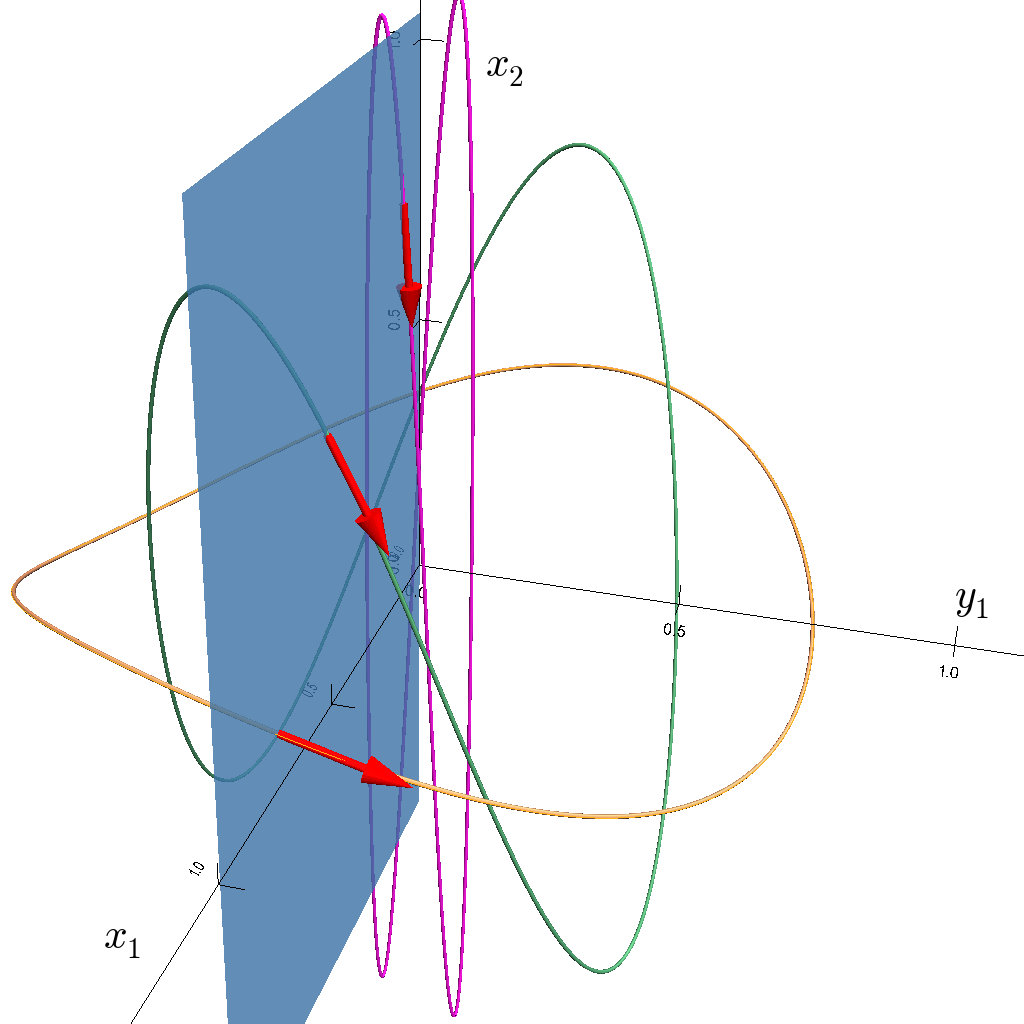
\includegraphics[width=0.45\textwidth]{BBgorbitsandslice}
\caption{$\SOn{2}$ Group orbits of $(0.75, 0, 0.1, 0.1)$ (orange), $(0.5, 0, 0.5, 0.5)$ (green)
$(0.1, 0, 0.75, 0.75)$ (pink) of two Fourier modes and the first mode \slicePlane\
projected on three dimensions. 3D projections of the group tangents at the
intersections with the \slicePlane\ are shown as red arrows. 
\BBedit{THIS FIGURE WAS GENERATED WITH LEFT HANDED ROTATION MATRIX,
NEEDS TO BE FIXED}}
\label{fig:BBgorbitsandslice}
\end{figure}

In section \ref{s-slice}, we explained the general procedure for reducing
the \SOn{2} symmetry by \mslices , here, we are going to focus on its 
geometrical interpretation by narrowing the consideration down to the \twoMode\ 
system. The \slice\ defined by \refeq{firstmodetemp} and the direction
constraint $x_1 > 0$ fixes the phase of the first complex Fourier mode to $0$;
and the \statesp\ points are related to their \slice\ ``representatives''
by the following $\Un{1}$ action:
\beq
	\sspRedC_n = e^{-\ii n \phi_1} \sspC_n \, .
\ee{e-1stmodeTransform}
We immediately see that the reconstruction phase in \refeq{eq:so2reduced}
is, for this particular \slice , the phase of the first mode without the
symmetry reduction. The relation \refeq{e-1stmodeTransform} provides us
another interpretation for the \sliceBord :  For the template \refeq{firstmodetemp},
\sliceBord\ condition \refeq{ChartBordCond} yields, 
$|\sspRedC_1| = |\sspC_1| = 0$, this means that the phase of the first Fourier
mode is not defined, hence the transformation \refeq{e-1stmodeTransform}
has no meaning. We illustrated this by drawing the $3D$ projections of the 
group orbits, and group tangents of three reduced \statesp\ points in 
\reffig{fig:BBgorbitsandslice}. Note, in \reffig{fig:BBgorbitsandslice} 
that as the magnitude of the first mode, $\sqrt{x_1^2 + y_1^2}$, relative
to that of the second mode becomes smaller, its respective group tangent 
has a larger component that lies within the \slice ; \sliceBord\ condition
\refeq{ChartBordCond} is satisfies when the group tangent is entirely in the \slice .

An immediate generalization of the transformation \refeq{e-1stmodeTransform},
can be fixing the phase of the higher Fourier modes; this, however, requires
some extra care as we shall explain for the second Fourier mode next.
Consider the phase-fixing transformation,
\beq
	\sspRedC_n = e^{-\ii n \phi_2/2} \sspC_n \, ,
	\label{e-2ndmodeTransform}
\eeq
which would fix the phase of $\sspRedC_2$ to $0$. Note, however, that 
$\phi_2 \in (0, 2 \pi]$ in can have discontinuities of $2 \pi$, and this 
would translate to the transformation of the first Fourier mode by \refeq{e-2ndmodeTransform} 
as a phase discontinuity of $\pi$. This discontinuity can be fixed by another 
transformation: 
\bea
	\tilde{\sspC}_1 &=& e^{-\ii 2 \hat{\phi}_1} |\sspRedC_1 | \, , \continue
	\tilde{\sspC}_{n \neq 1} &=& \sspRedC_n \, ,
	\label{e-PhaseDoubling}
\eea
where we simply doubled the phase $\hat{\phi}_1$ of the symmetry-reduced 
first mode $\sspRedC_1$, obtained by \refeq{e-2ndmodeTransform} and left
the rest of the modes unchanged. Combination of \refeq{e-2ndmodeTransform}
and \refeq{e-PhaseDoubling} is a valid symmetry reduction scheme since every 
group orbit is represented by a single point, furthermore, it is also continuous
and revertible hence one can make further computations, such as constructing
Poincar\'{e} sections, using this form. For the 2-mode case at hand, representation
\refeq{e-PhaseDoubling} does not have any particular advantage against 
\refeq{e-1stmodeTransform}, however, for higher dimensional flows, second 
(or higher) Fourier mode subspaces can have dynamical importance as shown in 
\refref{SCD07}. In order to capture those regions of the \statesp\ this 
representation would be a useful alternative.

\subsection{Polar coordinates}
\label{s-polar}

In \refref{PoKno05}, a polar coordinate representation of \refeq{eq:DangSO2}  
is obtained by defining the $\LieEl$-invariant phase: $\Phi = \phi_2 - 2 \phi_1$
and three symmetry invariant coordinates $(r_1, r_2 \cos \Phi, r_2 \sin \Phi)$.
One can see by direct comparison with \refeq{e-1stmodeTransform}, which 
yields $\sspRedC_1 = r_1$ and $\sspRedC_2 = r_2 e^{\ii \Phi}$, that this 
representation is a special case $(m=2)$, of the \slice\ defined by 
\refeq{firstmodetemp}. Corresponding ODEs for the polar representation 
were obtained in \refref{PoKno05} by  chain rule and substitution. Note 
that \mslices\ provides a general form \refeq{e-so2red1stmode} for symmetry 
reduced time evolution 
